\documentclass[output=paper,
modfonts,
newtxmath,
hidelinks,
]{langscibook} 

% \papernote{\footnotesize\normalfont
% Guillaume Enguehard. A thought on the form and the substance of Russian vowel reduction. To appear in: Denisa Lenertová, Roland Meyer, Radek Šimík \& Luka Szucsich (eds.), \textit{Advances in formal Slavic linguistics 2016}. Berlin: Language Science Press. [preliminary page numbering]
% }

%\setcounter{chapter}{4}

\title{A thought on the form and the substance of Russian vowel reduction}

\author{%
Guillaume Enguehard\affiliation{Université d’Orléans, CNRS/LLL}
}

% \chapterDOI{} %will be filled in at production
% \epigram{}

\abstract{\sloppy
This paper is an attempt to formalize the Russian vowel reduction within a substance-free approach. My contribution consists in arguing that Russian vowel reduction is a strict quantitative phenomenon (not a qualitative phenomenon). Finally, I propose a motivation based on the representation of stress in different autosegmental frameworks.

\keywords{Russian vowel reduction, phonology, substance-free, Element Theory}
}

\begin{document}
\maketitle
\shorttitlerunninghead{A thought on the form and the substance of Russian vowel reduction}

\begin{quotation}
\begin{raggedleft}
[\dots] our mission is closer to one of revelation than of perfection.\\\hfill\citep[132]{Hamilton1980}
\end{raggedleft}
\end{quotation}



\section{Introduction}


  Russian vowel reduction is known to be a complex mechanism showing strong variations both in the realization and the neutralization of vowel phonemes. This paper is a modest contribution to the understanding of this phenomenon. My aim is to stress the difference between the \textsc{substance} and the \textsc{form} of Russian vowel reduction. In the line of \citeauthor{Hjelmslev1943} (\citeyear{Hjelmslev1943}/\citeyear{Hjelmslev1971}), I will assume a clear separation between the realization of distinctive units (which I call \textsc{substance} or \textsc{phonetics}) and their abstract relations (which I call \textsc{form} or \textsc{phonemics}). Such a strong dichotomy was also recently renewed in \citet{Hale-Reiss2000} and \citet{Dresher2008} (among others). The aim of this paper is not to compete on the same field as very valuable studies addressing the realization of Russian unstressed vowels (e.g. \citealt{Crosswhite2000a,Crosswhite2000b}; \citealt{Padgett2004}; among others). These deal with phonetic realizations which are not central to the present paper. I rather propose a parallel -- substance-free -- approach suggesting that the form of Russian vowel reduction is more consistent than its phonetic realization. More specifically, I argue that Russian vowel reduction can be interpreted as a quantitative phenomenon motivated by a length distinction between stressed and unstressed syllables.

In \sectref{5:s2}, I introduce the various substantial and formal manifestations of Russian vowel reduction. In \sectref{5:s3}, I propose to analyze Russian vowel reduction as a quantitative -- rather than qualitative -- phenomenon. Finally, in \sectref{5:s4}, I suggest that this quantitative phenomenon can be motivated by the representation of stress in some autosegmental frameworks.

\section{The variation of Russian vowel reduction}\label{5:s2}

Russian phonological inventory has five vowel phonemes in stressed syllables \REF{5:1}. Following \citet[§19]{Garde1998}, I admit that [i] and [ɨ] are allophones of the same distinctive unit /i/: [ɨ] occurs after hard consonants (except velars) and [i] occurs elsewhere (\citealt{Avanesov1968}: §8; \citealt{Garde1998}: §95). The definition of vowel phonemes in terms of acoustic or articulatory features is not relevant for the substance-free approach advocated in this paper. For the time being, I simply define e.g. /i/ as a variable with relational properties $\neg$/u/, $\neg$/a/, $\neg$/e/ and $\neg$/o/.\footnote{\label{5:fn1}I use the negation symbol $\neg$ in order to represent oppositions: $x=\neg y$ should be read as $x\oplus y$ or “$x$ is right only if $y$ is wrong.”}

\ea \textbf{Russian stressed vowels}\label{5:1}\\\medskip
\begin{tabular}{|P{1.7cm}|P{1.7cm}|}
\hline
/i/&/u/\\\hline
/e/&/o/\\\hline
\multicolumn{2}{|c|}{/a/}\\\hline
\end{tabular}
\z

\noindent The inventory in \REF{5:1} undergoes a vowel reduction process in unstressed syllables. This process is manifested by (i) a phonetic difference between stressed and unstressed vowels and (ii) a neutralization of some phonological oppositions. Furthermore, both these substantial and formal aspects can vary according to the factors in \REF{5:2}.

\ea\label{5:2}\ea prosodic context
\ex segmental context
\ex morphological context
\ex dialectal context
\z\z

\subsection{Phonological factors}\label{5:s2.1}

Russian vowel reduction is conditioned by two phonological factors: (i) the segmental context (after hard consonants vs. soft consonants vs. \textit{š}, \textit{ž} or \textit{ts}) and (ii) the prosodic context (first pretonic syllable vs. non-pretonic syllables).\footnote{Soft consonants are palatal or palatalized consonants. Hard consonants are non-palatal or non-palatalized consonants. Consonants \textit{š}, \textit{ž} and \textit{ts} belong to a third category.} I base the following description on the Standard Russian variety depicted in \citet{Avanesov1968} and \citeauthor{Garde1980} (\citeyear{Garde1980}/\citeyear{Garde1998}).

\subsubsection{After hard consonants}\label{5:s2.1.1}

Russian vowel reduction after a hard consonant is illustrated in \REF{5:3}. In substantial (i.e. phonetic) terms, we observe a centralization of /a/ and /o/. The resulting vowel is realized as [ɐ] in the first pretonic syllable \REF{5:3a} and [ə] in other pretonic syllables \REF{5:3b} or in post-tonic syllables \REF{5:3c}.\footnote{However, a word-initial non pretonic /a/ or /o/ is unexpectedly realized as [ɐ] (e.g. [ɐ]tdavát’ ‘to give back’; see \citealt{Avanesov1968}: §14), not [ə].} Vowels /i/ and /u/ never reduce \citep[38--42]{Avanesov1968}.\footnote{Default grammatical information (such as nominative or singular) is not glossed.}\vspace{-\baselineskip}

\ea\label{5:3}\begin{multicols}{2}
\begin{xlist}
\exi{} \textbf{Stressed}
\ex gl[ˈa]z \tabto{2.1cm}‘eye’\label{5:3a}
\exi{} n[ˈɔ]g-i \tabto{2.1cm}‘legs, feet’
\ex st[ˈa]r-yj \tabto{2.1cm}‘old’\label{5:3b}
\exi{} g[ˈɔ]rod \tabto{2.1cm}‘city’
\ex šl-[ˈa] \tabto{2.1cm}‘walked.\textsc{f}’\label{5:3c}
\exi{} šl-[ˈɔ] \tabto{2.1cm}‘walked.\textsc{n}’
\end{xlist}\columnbreak
\begin{xlist}
\exi{} \textbf{Unstressed}
\exi{} gl[ɐ]z-á \tabto{2.1cm}‘eye’
\exi{} n[ɐ]g-á \tabto{2.1cm}‘leg, foot’
\exi{} st[ə]r-ik-á \tabto{2.1cm}‘old man.\textsc{gen}’
\exi{} g[ə]rod-á \tabto{2.1cm}‘cities’
\exi{} upál-[ə] \tabto{2.1cm}‘fell.\textsc{f}’ 
\exi{} upál-[ə] \tabto{2.1cm}‘fell.\textsc{n}’
\end{xlist}
\end{multicols}
\z

In formal (i.e. phonemic) terms, the two centralization processes illustrated in \REF{5:3a} and \REF{5:3b}/\REF{5:3c} result in the same neutralization of /a/ and /o/, represented by the merged box in \REF{5:4}. The place of /e/ (gray box) in this reorganization cannot be determined. Lexically, a stressed /e/ never occurs after a hard consonant \citep[§103]{Garde1998}. Even in (rare) loanwords, it never alternates with an unstressed vowel (e.g. \textit{mér, mér-a, mér-u, mér-om, mér-e, mér-y,} etc. ‘mayor’). Regardless the place of /e/, the Russian vowel inventory is reduced to three distinctive units in unstressed context.\largerpage[-2]

\ea \textbf{Vowel reduction after hard consonants (Standard Russian)}\label{5:4}\\\medskip
\begin{tabular}{|p{1.7cm}|p{1.7cm}|ll}
\cline{1-2}
\multicolumn{1}{|c|}{[ɨ]\textsuperscript{a}, [i]\textsuperscript{b}}&\multicolumn{1}{|c|}{[u]}&a.&after a hard consonant (except velars)\\\hhline{--~~}
\multicolumn{1}{|c|}{\shadecell}&\multicolumn{1}{|c|}{\multirow{2}{*}{[ɐ]\textsuperscript{c}, [ə]\textsuperscript{d}}}&b.&after a velar and in initial position\\\cline{1-1}
\multicolumn{1}{|p{1.7cm}}{}&&c.&in first pretonic syllable\\\cline{1-2}
\multicolumn{2}{c}{}&d.&in other unstressed syllables\\
\end{tabular}
\z


\subsubsection{After soft consonants}\label{5:s2.1.2}

Russian vowel reduction after a soft consonant is illustrated in \REF{5:5}. Substantially, /a/, /o/ and /e/ are fronted and raised to [i] in first pretonic \REF{5:5a}, in other pretonic syllables \REF{5:5b}, and in post-tonic syllables \REF{5:5c}.\vspace{-\baselineskip}

\ea\label{5:5}\begin{multicols}{2}
\begin{xlist}
\exi{} \textbf{Stressed}
\ex p’[ˈa]t’ \tabto{2.1cm}‘five’\label{5:5a}
\exi{} n’[ˈɔ]s \tabto{2.1cm}‘carried.\textsc{m}’
\exi{} l’[ˈɛ]s \tabto{2.1cm}‘forest’
\ex č’[ˈa]s \tabto{2.1cm}‘hour’\label{5:5b}
\exi{} č’[ˈɔ]rn-yj \tabto{2.1cm}‘black.\textsc{m}’
\exi{} b’[ˈɛ]dn-yj \tabto{2.1cm}‘poor.\textsc{m}’
\ex t’[ˈa]-n-ut \tabto{2.1cm}‘they pull’\label{5:5c}
\exi{} v’es’[ˈɔ]l-yj \tabto{2.1cm}‘happy.\textsc{m}’
\exi{} s’[ˈɛ]d \tabto{2.1cm}‘grey-haired.\textsc{m}’
\end{xlist}\columnbreak
\begin{xlist}
\exi{} \textbf{Unstressed}
\exi{} p’[i]t-ók \tabto{2.1cm}‘set of five’
\exi{} n’[i]s-ú \tabto{2.1cm}‘I carry’
\exi{} l’[i]s-ók \tabto{2.1cm}‘wood’
\exi{} č’[i]s-ov-ój \tabto{2.1cm}‘hourly.\textsc{m}’
\exi{} č’[i]rn-ov-ík \tabto{2.1cm}‘draft’
\exi{} b’[i]dn-otá \tabto{2.1cm}‘poor person’
\exi{} vý-t’[i]-n-u \tabto{2.1cm}‘I will pull out’
\exi{} v’és’[i]l-o \tabto{2.1cm}‘happily’
\exi{} pró-s’[i]d’ \tabto{2.1cm}‘graying hair’
\end{xlist}
\end{multicols}
\z

\noindent Formally, the opposition between /a/, /e/, /o/ and /i/ is neutralized both in pretonic and non pretonic syllables \REF{5:6}. It results that the Russian vowel inventory is reduced to two distinctive units in this context.

\ea \textbf{Reduced vowels after soft consonants (Standard Russian)}\label{5:6}\\\medskip
\begin{tabular}{|p{1.7cm}p{1.7cm}|}
\hline
&\multicolumn{1}{|c|}{[u]}\\\cline{2-2}
\multicolumn{1}{|c}{[i]}&\\
&\\\hline
\end{tabular}
\z

\subsubsection{After \textit{š, ž,} and \textit{ts}}\label{5:s2.1.3}

Russian vowel reduction after \textit{š, ž,} and \textit{ts} is represented in \REF{5:7}. Substantially, /a/ is centralized to [ɐ] in pretonic syllables \REF{5:7a} and [ə] in non pretonic syllables \REF{5:7b}. As for /o/ and /e/, they are centralized to [ɨ] in pretonic syllables \REF{5:7c} and [ə] in non pretonic syllables \REF{5:7d}.%\vspace{-\baselineskip}

% \newpage
\ea\label{5:7}\begin{multicols}{2}
\begin{xlist}
\exi{} \textbf{Stressed}
\ex ž[ˈa]rk-ij \tabto{2.1cm}‘hot.\textsc{m}’\label{5:7a}
\ex loš[ˈa]d-k-a \tabto{2.1cm}‘little horse’\label{5:7b}
\ex ž[ˈɔ]n \tabto{2.1cm}‘wife.\textsc{gen.pl}’\label{5:7c}
\exi{} ts[ˈɛ]n \tabto{2.1cm}‘price.\textsc{gen.pl}’
\ex ž[ˈɔ]lt-yj \tabto{2.1cm}‘yellow.\textsc{m}’\label{5:7d}
\exi{} ts[ˈɛ]l-yj \tabto{2.1cm}‘whole.\textsc{m}’
\end{xlist}\columnbreak
\begin{xlist}
\exi{} \textbf{Unstressed}
\exi{} ž[ɐ]r-á \tabto{2.1cm}‘heat’
\exi{} lóš[ə]d’ \tabto{2.1cm}‘horse’
\exi{} ž[ɨ]n-á \tabto{2.1cm}‘wife’
\exi{} ts[ɨ]n-á \tabto{2.1cm}‘price’
\exi{} ž[ə]lt-izn-á \tabto{2.1cm}‘yellowness’
\exi{} ts[ə]l-ik-óm \tabto{2.1cm}‘entirely’
\end{xlist}
\end{multicols}
\z

\noindent Formally, the mechanisms observed in pretonic and non pretonic syllables are distinct. In pretonic syllables, a neutralization applies between /e/, /o/ and /i/ \REF{5:8a}. In non-pretonic syllables, a neutralization applies between /a/, /e/ and /o/ \REF{5:8b}. In both cases, it results that the Russian vowel inventory is reduced to three distinctive units.

\ea \textbf{Reduced vowels after \textit{š, ž, ts} (Standard Russian)}\label{5:8}\vspace{-8pt}\begin{multicols}{2}
\ea Pretonic\label{5:8a}\\\medskip
\begin{tabular}{|P{1.7cm}P{1.7cm}|}
\hline
\multirow{2}{*}{[ɨ]}&\multicolumn{1}{|c|}{[u]}\\\cline{2-2}
&\\\hline
\multicolumn{2}{|c|}{[ɐ]}\\\hline
\end{tabular}\columnbreak
\ex Non-pretonic\label{5:8b}\\\medskip
\begin{tabular}{|P{1.7cm}|P{1.7cm}|}
\hline
[ɨ]&[u]\\\hline
\multicolumn{2}{|c|}{\multirow{2}{*}{[ə]}}\\
\multicolumn{2}{|c|}{}\\\hline
\end{tabular}
\z
\end{multicols}
\z

\subsection{Morphological factors}\label{5:s2.2}

The reduction patterns observed in inflectional suffixes (only after soft consonants and \textit{š}, \textit{ž} or \textit{ts}) differ from the generalizations of \sectref{5:s2.1.2} and \sectref{5:s2.1.3}, both substantially and formally.


Substantially, /a/ and /o/ are centralized to [ə] after soft consonants \REF{5:9a} and \textit{š}, \textit{ž} or \textit{ts} \REF{5:9b}. As for /e/, it is raised to [i] after a soft consonant \REF{5:9c}, and [ɨ] after \textit{š}, \textit{ž} or \textit{ts} \REF{5:9d}.\vspace{-\baselineskip}

\ea\label{5:9}\begin{multicols}{2}
\begin{xlist}
\exi{} \textbf{Stressed}
\ex z’eml’-[ˈa] \tabto{2.1cm}‘earth.\textsc{f}’\label{5:9a}
\exi{} b’el’j-[ˈɔ] \tabto{2.1cm}‘linen.\textsc{n}’
\ex duš-[ˈa] \tabto{2.1cm}‘soul.\textsc{f}’\label{5:9b}
\exi{} kol’ts-[ˈɔ] \tabto{2.1cm}‘ring.\textsc{n}’
\ex b’el’j-[ˈɛ] \tabto{2.1cm}‘linen.\textsc{loc}’\label{5:9c}
\ex kol’ts-[ˈɛ] \tabto{2.1cm}‘ring.\textsc{loc}’\label{5:9d}
\end{xlist}\columnbreak
\begin{xlist}
\exi{} \textbf{Unstressed}
\exi{} dýn’-[ə] \tabto{2.1cm}‘melon.\textsc{f}’
\exi{} pól’-[ə] \tabto{2.1cm}‘field.\textsc{n}’
\exi{} súš-[ə] \tabto{2.1cm}‘dry land.\textsc{f}’
\exi{} lóž-[ə] \tabto{2.1cm}‘couch.\textsc{n}’
\exi{} pól’-[i] \tabto{2.1cm}‘field.\textsc{loc}’
\exi{} lóž-[ɨ] \tabto{2.1cm}‘couch.\textsc{loc}’
\end{xlist}
\end{multicols}
\z

\noindent These reduction patterns have the same formal representation after a soft consonant and after \textit{š}, \textit{ž} or \textit{ts} \REF{5:10}. A neutralization applies (i) between /i/ and /e/ and (ii) between /a/ and /o/. Again, it results that the Russian vowel inventory is reduced to three distinctive units in these contexts.

\ea \textbf{Reduced vowels in inflectional suffixes}\label{5:10}\\\medskip
\begin{tabular}{|P{1.7cm}|P{1.7cm}|ll}
\cline{1-2}
\multirow{2}{*}{[ɨ]\textsuperscript{a}, [i]\textsuperscript{b}}&[u]&a.&after a soft consonant\\\cline{2-2}
&\multirow{2}{*}{[ə]}&b.&after \textit{š, ž,} or \textit{ts}\\\cline{1-1}
\multicolumn{2}{|c|}{}&&\\\cline{1-2}
\end{tabular}
\z


\subsection{Dialectal factors}\label{5:s2.3}

The reduction patterns described above concern the Standard Russian variety and are not shared by all dialects. In what follows, I give a brief overview of relevant dialectal features concerning the phonology of unstressed vowels.

Concerning the phonology of unstressed vowels after a hard consonant, Russian dialects can be divided into three groups: dialects with \textsc{Akanye} \citep[§47]{Avanesov1949}, dialects with \textsc{Okanye} \citep[§42]{Avanesov1949}, and dialects with \textsc{Ukanye} \citep[§43]{Avanesov1949}; see \REF{5:11}. I do not discuss subtypes such as varieties with \textsc{Dissimilative Akanye} \citep[§49]{Avanesov1949} and \textsc{Mixed Okanye-Akanye} \citep[§46]{Avanesov1949}.

\ea \textbf{Dialectal variations after a hard consonant}\label{5:11}
\ea \textsc{Akanye:} neutralization of /a/ and /o/
\ex \textsc{Okanye:} no neutralization of /a/ and /o/
\ex \textsc{Ukanye:} neutralization of /o/ and /u/
\z\z

\noindent Concerning the phonology of unstressed vowels after a soft consonant, Russian dialects can be divided into three other groups: dialects with \textsc{Yakanye} \citep[§60]{Avanesov1949}, dialects with \textsc{Okanye} \citep[§56]{Avanesov1949}, and dialects with \textsc{Ikanye} \citep[§59]{Avanesov1949}; see \REF{5:12}. Subtypes such as varieties with \textsc{Ekanye} \citep[§57]{Avanesov1949} or \textsc{Dissimilative Yakanye} \citep[§64]{Avanesov1949} are not relevant to this paper.


\ea \textbf{Dialectal variations after a soft consonant}\label{5:12}
\ea \textsc{Yakanye:} neutralization of /a/, /o/, and /e/
\ex \textsc{Okanye:} no neutralization of /a/, /e/, and /o/
\ex \textsc{Ikanye:} neutralization of /a/, /o/, /e/, and /i/
\z\z

\noindent A schematic geographical distribution of the dialectal features in \REF{5:11} and \REF{5:12} are represented in \figref{5:f1} (source: \citealt{Bukrinskaja-etal1994}).

\begin{figure}
\subfigure[After a hard consonant\label{5:f1a}]{
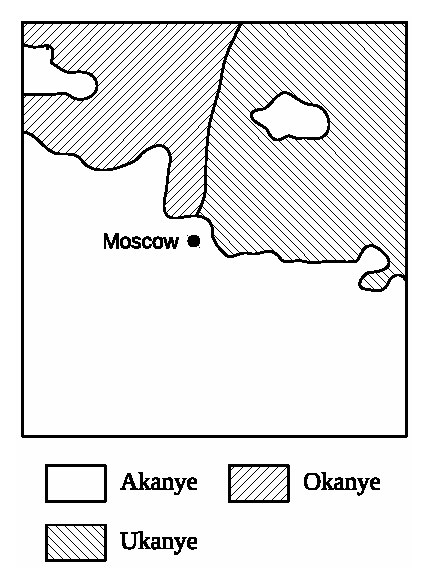
\includegraphics[height=0.3\textheight]{figures/05enguehard_f1.eps}
}
\subfigure[After a soft consonant\label{5:f1b}]{
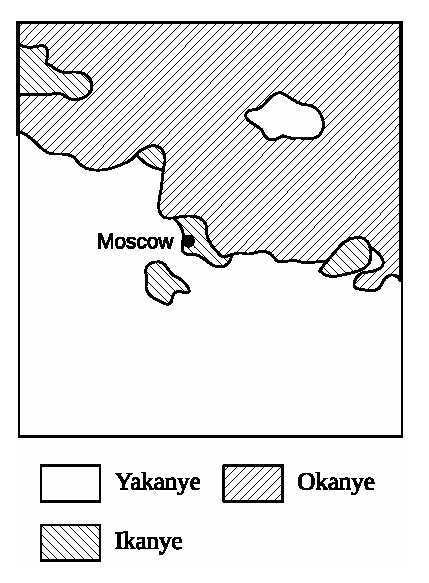
\includegraphics[height=0.3\textheight]{figures/05enguehard_f2.eps}
}
\caption{Distribution of dialectal variants of Russian vowel reduction}\label{5:f1}
\end{figure}

Dialects with proper Okanye have no vowel reduction (some subtypes can show some neutralizations in specific segmental contexts; see \citealt[§46, §56]{Avanesov1949}). Akanye and Ikanye refer to the reduction patterns illustrated in \REF{5:4} and \REF{5:6} respectively. In what follows, I address the remaining Ukanye and Yakanye patterns.

\subsubsection{Ukanye}\label{5:s2.3.1}

Substantially, Ukanye is manifested by a raising of /o/ in both first pretonic syllables \REF{5:13a} and other pretonic syllables \REF{5:13b}. A raising of /o/ can also be found in post-tonic syllables of several central and southern dialects \citep[§104]{Avanesov1949} or in the Kamtchatka dialect (see \citealt[40]{Gluschenko2007}).\vspace{-8pt}

\ea\label{5:13}\begin{multicols}{2}
\begin{xlist}
\exi{} \textbf{Stressed}
\ex d[ˈɔ]m \tabto{2.1cm}‘house’\label{5:13a}
\exi{} x[ˈɔ]lod \tabto{2.1cm}‘coldness’
\ex g[ˈɔ]lub’ \tabto{2.1cm}‘dove’\label{5:13b}
\exi{} {[ˈɔ]strov} \tabto{2.1cm}‘island’
\end{xlist}\columnbreak
\begin{xlist}
\exi{} \textbf{Unstressed}
\exi{} d[u]m-ój \tabto{2.1cm}‘home’
\exi{} x[u]lód-n-yj \tabto{2.1cm}‘cold.\textsc{m}’
\exi{} g[u]lub’-éj \tabto{2.1cm}‘dove.\textsc{gen.pl}’
\exi{} {[u]strov-á} \tabto{2.1cm}‘islands’
\end{xlist}
\end{multicols}
\z

\noindent Formally, this raising results in a reorganization of the vowel inventory into three distinctive units, due to the neutralization of the opposition between /o/ and /u/.

\ea \textbf{Ukanye}\label{5:14}\\\medskip
\begin{tabular}{|P{1.7cm}|P{1.7cm}|}
\hline
[ɨ]&\multirow{2}{*}{[u]}\\\hhline{-~}
\shadecell{}&\\\hline
\multicolumn{2}{|c|}{[a]}\\\hline
\end{tabular}
\z


\subsubsection{Yakanye}\label{5:s2.3.2}

Yakanye is substantially manifested by a lowering of /o/ and /e/ after a soft consonant in pretonic syllables \REF{5:15}. Such a lowering of /o/ and /e/ can also be found in other pretonic syllables (see \citealt[§96]{Avanesov1949}) and in post-tonic syllables (\citealt[§108--112]{Avanesov1949}) of several central and southern dialects.\footnote{The variation of post-tonic vowels is known to be very complex due to, e.g., morphological factors \citep[§107]{Avanesov1949}. Thus, it is only mentioned here.}\vspace{-\baselineskip}

\ea\label{5:15}\begin{multicols}{2}
\begin{xlist}
\exi{} \textbf{Stressed}
\exi{} p’[ˈa]t’ \tabto{2.1cm}‘five’
\exi{} n’[ˈɔ]s \tabto{2.1cm}‘carried.\textsc{m}’
\exi{} l’[ˈɛ]s \tabto{2.1cm}‘forest’
\end{xlist}\columnbreak
\begin{xlist}
\exi{} \textbf{Unstressed}
\exi{} p’[a]t-ók \tabto{2.1cm}‘set of five’
\exi{} n’[a]s-ú \tabto{2.1cm}‘I carry’
\exi{} l’[a]s-ók \tabto{2.1cm}‘wood’
\end{xlist}
\end{multicols}
\z

\noindent Formally, this lowering also results in a reorganization of the vowel inventory into three distinctive units, due to the neutralization of the opposition between /a/, /o/, and /e/.

\ea \textbf{Yakanye}\label{5:16}\\\medskip
\begin{tabular}{|P{1.7cm}|P{1.7cm}|}
\hline
[i]&[u]\\\hline
\multicolumn{2}{|c|}{\multirow{2}{*}{[a]}}\\
\multicolumn{2}{|c|}{}\\\hline
\end{tabular}
\z


\subsection{Summary}\label{5:s2.4}

To conclude this section, we saw that the Russian vowel inventory is reduced to three distinctive units in unstressed syllables (except after a soft consonant in dialects with Ikanye; see \REF{5:6}). These three distinctive units are represented with /A/, /I/ and /U/ in \REF{5:17}.\footnote{These symbols do not correspond to phonetic properties. They could be represented with features {\textbar}A{\textbar}, {\textbar}B{\textbar}, and {\textbar}C{\textbar}, or {\textbar}X{\textbar}, {\textbar}Y{\textbar}, and {\textbar}Z{\textbar}, etc.}

\ea \textbf{Russian unstressed vowels}\label{5:17}\\\medskip
\begin{tabular}{|P{1.7cm}|P{1.7cm}|}
\hline
/I/&/U/\\\hline
\multicolumn{2}{|c|}{/A/}\\\hline
\end{tabular}
\z

\noindent Now, if we assume that distinctive units are exclusively defined by a set of abstract relational properties, then the three distinctive units found in unstressed context \REF{5:17} should not be assimilated to a subset of the five distinctive units found in stressed context \REF{5:1}. Each distinctive unit of the stressed context is defined by a set of oppositions to four other units (e.g. /i/${}=\neg{}$/u/, $\neg$/a/, $\neg$/e/, $\neg$/o/). But each distinctive unit found in unstressed context \REF{5:17} is defined by a set of oppositions to two other units only (e.g. /I/ = $\neg$/U/, $\neg$/A/). In that sense, /I/, /A/, and /U/ are less specified than /i/, /e/, /a/, /o/, or /u/. They thus represent \textsc{archiphonemes}. This notion will be discussed and defined below.

I suggest that the main formal aspect of Russian vowel reduction lies in this \textit{underspecification} of vowel phonemes, not in the realizations that result from this underspecification.

\section{Formal representation of Russian vowel reduction}\label{5:s3}\largerpage[2]

\begin{table}[b]
\caption{Alternation between stressed vowels and their underspecified counterparts}
\label{5:t1}
\begin{tabularx}{\textwidth}{P{1.5cm}P{1.35cm}P{1.35cm}P{1.35cm}P{1.35cm}P{1.35cm}P{1.35cm}}
\lsptoprule
\textbf{Stressed} & \multicolumn{6}{c}{\textbf{Unstressed}}\\\midrule
&\textbf{Type A}&\textbf{Type B}&\textbf{Type C}&\textbf{Type D}&\textbf{Type E}&\textbf{Type F}\\
&\REF{5:4}&\REF{5:6}&\REF{5:8a}&\REF{5:8b}, \REF{5:16}&\REF{5:10}&\REF{5:14}\\\midrule
/a/ & /A/ & /I/ & /A/ & /A/ & /A/ & /A/\\
/e/ & -- & /I/ & /I/ & /A/ & /I/ & --\\
/o/ & /A/ & /I/ & /I/ & /A/ & /A/ & /U/\\
/i/ & /I/ & /I/ & /I/ & /I/ & /I/ & /I/\\
/u/ & /U/ & /U/ & /U/ & /U/ & /U/ & /U/\\
\lspbottomrule
\end{tabularx}
\end{table}

In a substance-free approach, it could be tempting to interpret Russian vowel reduction as a simple redistribution of the five vowel phonemes into a reduced ternary inventory. Following such a hypothesis, every stressed vowel could freely alternate with every archiphoneme of the unstressed context. But this is not the case.

\tabref{5:t1} outlines the various alternations between stressed vowels and their underspecified counterparts in unstressed syllables. It can be observed that these alternations are constrained: e.g., /i/ and /u/ never alternate with the same archiphoneme. In order to formalize this constraint, we need to distinguish the behaviors of vowel phonemes by referring to their respective properties.

I propose to determine the formal properties of vowel phonemes based on the definition of archiphonemes in \REF{5:18}. According to this definition, two phonemes can alternate with the same archiphoneme iff they share a relevant feature. Thus, if /i/ and /u/ never alternate with the same archiphoneme, we can suppose that they do not share any relevant feature. The issue is that /i/ and /u/ seem to share some distinctive properties. Substantially, /i/ and /u/ are [$+$high]. Formally, they share relational properties such as $\neg$/a/, $\neg$/e/, and $\neg$/o/.%\largerpage[-1]

\ea \textbf{Definition of the archiphoneme} \citep[201]{Akamatsu1988}\label{5:18}\\
The archiphoneme is a distinctive unit whose phonological content is identical with the relevant features common to the member phonemes of a neutralizable opposition, which is distinct from any of these member phonemes and which occurs in the position of neutralization.
\z

\noindent One possible solution is to assume that the relational properties of phonemes are primitively organized into indivisible sets (e.g. \{$\neg$/a/, $\neg$/u/, $\neg$/o/, $\neg$/e/\} for /i/ and \{$\neg$/a/, $\neg$/i/, $\neg$/o/, $\neg$/e/\} for /u/). In this trivial example, /i/ and /u/ do not share any property. Such a representation of distinctive features by means of complex sets is defended in several models like, e.g., Particle Phonology \citep{Schane1984} or Element Theory \citep{Kaye-etal1985}. Element Theory assumes that distinctive features are organized into complex properties represented by {\textbar}A{\textbar}, {\textbar}I{\textbar} and {\textbar}U{\textbar}.\footnote{A substance-free reinterpretation of these features could be \{$\neg${\textbar}I{\textbar}, $\neg${\textbar}U{\textbar}\}, \{$\neg${\textbar}A{\textbar}, $\neg${\textbar}U{\textbar}\} and \{$\neg${\textbar}I{\textbar}, $\neg${\textbar}A{\textbar}\} respectively.} Each vowel can be defined by one or several of these properties.

Thus, based on the alternations in \tabref{5:t1} (sketched in \figref{5:f3}) and the definition of archiphonemes in \REF{5:18}, it is now possible to determine the underlying representation of each stressed vowel in terms of abstract features {\textbar}A{\textbar}, {\textbar}I{\textbar}, and {\textbar}U{\textbar}, representing the indivisible properties of the three archiphonemes found in unstressed syllables.\footnote{Types B and C are not taken into account in this outline. They will be discussed below.}


% figure in (21) -> SEBASTIAN tikz 
\begin{figure}
\begin{tikzpicture}
\node [circle, draw, inner sep=7mm, outer sep=-7mm] (i) {/i/};
\node (e) [right=-1mm of i] {/e/};
\node [circle, draw, inner sep=7mm, outer sep=-7mm] (a) [right=-1mm of e] {/a/};
\node (o) [right=-1mm of a] {/o/};
\node [circle, draw, inner sep=7mm, outer sep=-7mm] (u) [right=-1mm of o] {/u/};

\node [below=of i] {/I/};
\node [below=of a] {/A/};
\node [below=of u] {/U/};


\end{tikzpicture}
\caption{Outline of the neutralizable relations between vowel phonemes}
\label{5:f3}
\end{figure}

First, we saw that the vowels /i/ and /u/ never alternate with the same archiphoneme. Thus it can be supposed that they do not share any property. For convenience, I represent the distinct properties of /i/ and /u/ with {\textbar}I{\textbar} and {\textbar}U{\textbar} respectively. Second, /e/ and /i/ can alternate with the same archiphoneme (Types B, C, E). Thus /e/ contains {\textbar}I{\textbar}. Third, /o/ and /u/ can alternate with the same archiphoneme (Type F). Thus /o/ contains {\textbar}U{\textbar}. Fourth, /e/, /o/ and /a/ can altogether alternate with an archiphoneme opposed to /I/ and /U/ (Types A, D). Thus they all share a property that is not {\textbar}I{\textbar} nor {\textbar}U{\textbar}. I represent this property with {\textbar}A{\textbar}. The resulting representation of stressed vowel is outlined in \REF{5:19}.

\ea \textbf{Representation of Russian vowels (preliminary version)}\label{5:19}\\\medskip
\begin{tabular}{|P{1.7cm}|P{1.7cm}|}
\hline
\textbar I\textbar&\textbar U\textbar\\\hline
\textbar AI\textbar&\textbar AU\textbar\\\hline
\multicolumn{2}{|c|}{\textbar A\textbar}\\\hline
\end{tabular}
\z

\noindent One can observe that /o/ and /a/ can also alternate with /i/ after a soft consonant, \textit{š}, \textit{ž} and \textit{ts} (Types B, C). Accordingly, we should assume that they both contain an {\textbar}I{\textbar}. However, this leads to an important issue: in this case, both /e/ and /a/ would be defined by {\textbar}IA{\textbar}. Fortunately, it can be argued that the {\textbar}I{\textbar} found in this context is inherited from the preceding consonants. From the substantial point of view, these are palatal or palatalized segments that trigger a fronting and a raising of /o/ and /a/ via assimilation. From the formal point of view, it is more difficult to argue that soft consonants share an {\textbar}I{\textbar} feature with the archiphoneme /I/. Nevertheless, I already mentioned that /e/ is lexically found after soft consonants only (see \sectref{5:s2.1.1}). In other words, /e/ contains a feature that neutralizes the opposition between hard and soft consonants. This feature can be {\textbar}I{\textbar} or {\textbar}A{\textbar}; see \REF{5:19}. The vowel /a/ can be indistinctly preceded by a soft or a hard consonant. However, there is a correlation between /i/ and the hard/soft contrast: e.g., the verbal suffix \textit{-i} always triggers a softening of the preceding consonant (e.g., \textit{bro}[s]\textit{{}-}\textit{át’} `throw.\textsc{ipfv}' vs. \textit{bro}[sʲ]\textit{{}-}\textit{ít’} ‘throw.\textsc{pfv}’). Thus, it can be supposed that the opposition between these two consonant classes is due to the presence of a property shared by /e/ and /i/, namely {\textbar}I{\textbar}.

The representation in \REF{5:19} raises another issue concerning the definition of archiphonemes. Following the definition \REF{5:18}, the result of a neutralization process is a \textit{new} phonological item defined by the set of relations common to the member phonemes of a neutralized opposition. In this respect, {\textbar}A{\textbar}, which is the representation of the archiphoneme /A/, cannot be the representation of the fully specified vowel /a/. Indeed, the phoneme /a/ has something more than the archiphoneme /A/: it contrasts with /e/ and /o/. This property should be represented by an additional feature in /a/ distinguishing it from /A/. The only possible feature, distinct from {\textbar}I{\textbar} in /e/, {\textbar}U{\textbar} in /o/ and \textit{zero} in /A/, is the {\textbar}A{\textbar} feature. Thus, if we want to represent the formal distinction between /a/ and /A/, we should assume that /a/ is a complex vowel made of two {\textbar}A{\textbar} features. Such a repetition of distinctive properties in the structure of vowels was already proposed in the Particle Theory of \citet{Schane1984}, developed in \citet{Carvalho1993,Carvalho1994}. Extending the same reasoning to the representation of /i/ and /u/, I now assume the representation of stressed and unstressed vowels in \REF{5:20a} and \REF{5:20b}, respectively.

\ea \textbf{Representation of Russian vowels (final version)}\vspace{-8pt}\label{5:20}\begin{multicols}{2}
\ea Stressed vowels\label{5:20a}\\\medskip
\begin{tabular}{|P{1.7cm}|P{1.7cm}|}
\hline
\textbar II\textbar&\textbar UU\textbar\\\hline
\textbar AI\textbar&\textbar AU\textbar\\\hline
\multicolumn{2}{|c|}{\textbar AA\textbar}\\\hline
\end{tabular}\columnbreak
\ex Unstressed vowels\label{5:20b}\\\medskip
\begin{tabular}{|P{1.7cm}|P{1.7cm}|}
\hline
\textbar I\textbar&\textbar U\textbar\\\hline
\multicolumn{2}{|c|}{\textbar A\textbar}\\\hline
\multicolumn{2}{c}{}
\end{tabular}
\z
\end{multicols}
\z

\noindent Following this representation, Russian vowel reduction can be interpreted as a quantitative phenomenon. Stressed vowel have more distinctive properties than unstressed vowels. I propose to represent this distinction with the rule in \REF{5:21a}. This rule purposefully does not refer to the quality of distinctive properties. Indeed, such an ambiguity is likely to derive variations. According to this mechanism, /e/ can be reduced to {\textbar}A{\textbar} \textit{or} {\textbar}I{\textbar}, and /o/ can be reduced {\textbar}A{\textbar} \textit{or} {\textbar}U{\textbar}. This parametrical choice depends on the phonological, morphological and dialectal contexts. In order to account for the regularity of this choice in a given language variety, I propose the principle in \REF{5:21b}. The term “configuration” refers to (i) the representation of a given segment and (ii) both its phonological and morphological contexts. As an example, a pretonic /a/ and a non-pretonic /a/ represent two distinct configurations. They may or may not have two different interpretations.

\ea \textbf{Principles of Russian vowel reduction (first attempt)}\label{5:21}
\ea Unstressed vowels lose a distinctive property.\label{5:21a}
\ex For a given speaker, a configuration A always has an interpretation B.\label{5:21b}
\z\z

\noindent The principle in \REF{5:21a} concerns the form of distinctive units, and the principle in \REF{5:21b} concerns the substance of distinctive units. Following \citet{Hjelmslev1936} (here cited from \citealt{Hjelmslev1973}), these principles refer to different components of the language: “phonematics” and “phonology”:

\begin{quotation}
One and the same phonematic system may be pronounced by means of very different phonological systems. \citep[159]{Hjelmslev1973}
\end{quotation}

The contribution of this analysis consisted in suggesting that Russian vowel reduction can be analyzed as a strict quantitative phenomenon if we do not refer to substance. In the following section, I suggest that this quantitative phenomenon can be motivated by the representation of stress.

\section{Motivation of Russian vowel reduction}\label{5:s4}

In the previous section, we saw that the formal representation of Russian vowel reduction is strictly a matter of complexity (i.e., quantity of information). But one can ask: Why should an unstressed vowel have less distinctive properties than a stressed vowel?

Interestingly, Russian vowel reduction is related to another quantitative phenomenon conditioned by stress: Russian stressed vowels are phonetically longer than unstressed vowels (\citealt{Zlatoustova1953}; \citealt{Vysotskij1973}; \citealt[47]{Al’muhamedova-Kul’sharipova1980}; \citealt[155--158]{Svetozarova1982}; \citealt[5--7]{Crosswhite2000a}; \citealt[116--117]{Crosswhite2000b}; \citealt[43]{Knjazev2006}). Such a correlation between stress and vowel length can be observed in several languages, and it was represented with an extra time unit provided by stress in \citet{Chierchia1986}, \citet{Larsen1998}, \citet{Segeral-Scheer2008}, \citet{Crosswhite2000a,Crosswhite2000b}, \citet{Bucci2013}, and \citet{Enguehard2016}, among others. In what follows, I represent this extra unit with an x-slot on the right of the stressed nucleus \REF{5:22}.\footnote{One could object that length belongs to the substance while stress belongs to the form. Alternatively, \citet{Enguehard2016} proposed that the relation between them could be inverted: stress is a possible substantial realization of length.}

\ea d[ˈɔ]m ‘house’\label{5:22}

\begin{tikzpicture}
\node(x1) {x\vphantom{]}};
\node(x2) [right=0mm of x1] {x\vphantom{]}};
\node(x3) [right=0mm of x2] {[x]};
\node(x4) [right=0mm of x3] {x\vphantom{]}};

\node(stress) [above=5mm of x3] {stress};

\node(d) [below=5mm of x1] {d};
\node(o) [below=5mm of x2] {o\vphantom{d}};
\node(m) [below=5mm of x4] {m\vphantom{d}};

\draw (x1) -- (d.north);
\draw (x2) -- (o.north);
\draw [dashed] (x3) -- (o.north);
\draw (x4) -- (m.north);

\draw[<->,thick] (x3) -- (stress);

\end{tikzpicture}
 
\z

\noindent The relation between vowel length and vowel reduction was already formalized in \citet{Crosswhite2000a,Crosswhite2000b}. \citeauthor{Crosswhite2000a} proposed that the sonority of vowels is conditioned by the presence of a mora in stressed and pretonic syllables. Here, I propose to take the additional step of unifying length and Russian vowel reduction with the following generalization: the amount of realized vowel features is proportional to the amount of available skeletal slots. If a vowel stands in a stressed position, it has two available slots and all its distinctive properties are manifested \REF{5:23a}. If a vowel stands in an unstressed position, it has one available slot and only one of its distinctive properties can be manifested \REF{5:23b}. It turns out that Russian mid vowels are abstractly represented as sorts of diphthongs.\footnote{Note that this would be an issue if Russian had \textit{real} diphthongs. But it does not have any.}

\begin{multicols}{2}
\ea \ea d[ˈɔ]m ‘house’\label{5:23a}

\begin{tikzpicture}
\node(x1) {x\vphantom{]}};
\node(x2) [right=0mm of x1] {x\vphantom{]}};
\node(x3) [right=0mm of x2] {[x]};
\node(x4) [right=0mm of x3] {x\vphantom{]}};

\node(d) [below=5mm of x1] {d};
\node(A) [below=5mm of x2] {A\vphantom{d}};
\node(U) [below=5mm of A] {U\vphantom{d}};
\node(m) [below=5mm of x4] {m\vphantom{d}};


\node(stress) [above=5mm of x3] {stress};

\draw (x1) -- (d.north);
\draw (x2) -- (A.north);
\draw[dashed,rounded corners] (x3) |- (U.east);
\draw (x4) -- (m.north);

\draw[<->,thick] (x3) -- (stress);

\end{tikzpicture}

\columnbreak
\ex d[ɐ]má ‘houses’\label{5:23b}
\begin{tikzpicture}
\node(x1) {x\vphantom{]}};
\node(x2) [right=0mm of x1] {x\vphantom{]}};
\node(x3) [right=0mm of x2] {x\vphantom{]}};
\node(x4) [right=0mm of x3] {x\vphantom{]}};
\node(x5) [right=0mm of x4] {[x]};

\node(stress) [above=5mm of x5] {stress};

\node(d)  [below=5mm of x1] {d};
\node(A1) [below=5mm of x2] {A\vphantom{d}};
\node(m)  [below=5mm of x3] {m\vphantom{d}};
\node(A2) [below=5mm of x4] {A\vphantom{d}};

\node(U)  [below=5mm of A1] {(U)};
\node(A3) [below=5mm of A2] {A\vphantom{)}};

\draw (x1) -- (d.north);
\draw (x2) -- (A1.north);
\draw (x3) -- (m.north);
\draw (x4) -- (A2.north);
\draw[dashed,rounded corners]   (x5.south) |- (A3.east) ;

\draw[<->,thick] (x5) -- (stress);

\end{tikzpicture}

\z\z
\end{multicols}

\noindent Note that the distinctive property that is manifested in \REF{5:23b} is not necessarily {\textbar}A{\textbar}. In a dialect with Ukanye, the realized property is {\textbar}U{\textbar} (e.g., \textit{d}[ɐ]\textit{mój} vs. \textit{d}[u]\textit{mój} ‘home’).

\section{Conclusion}\label{5:s5}

As a conclusion, this paper is an attempt to formalize Russian vowel reduction without referring to substance. I suggested that Russian vowel reduction does not handle the quality of vowel phonemes, but the quantity of their distinctive properties. Then, I proposed that the quantity of distinctive properties is conditioned by the quantity of skeletal slots. In that sense, Russian qualitative distinction between stressed and unstressed syllables is not very different from length distinctions observed in languages like Italian (see \citealt{Parmenter-Carman1932}). Such a generalization supposes an interesting convergence (for further studies) between paradigmatic and syntagmatic axes.


\section*{Abbreviations}

\begin{tabularx}{.5\textwidth}{@{}lQ@{}}
\textsc{f}&feminine\\
\textsc{gen}&genitive\\
\textsc{ipfv}&imperfective\\
\textsc{loc}&locative\\
\end{tabularx}%
\begin{tabularx}{.5\textwidth}{@{}lQ@{}}
\textsc{m}&masculine\\
\textsc{n}&neuter\\
\textsc{pfv}&perfective\\
\textsc{pl}&plural\\
\end{tabularx}

\sloppy
\printbibliography[heading=subbibliography,notkeyword=this]

\end{document}
